\documentclass{article}

\usepackage{graphicx}
\usepackage{amsmath}
\usepackage{siunitx}
\usepackage{float}
\usepackage{hyperref}
%\DeclareGraphicsExtensions{.png, .pdf}
\DeclareGraphicsExtensions{.pdf, .png, .jpg}

\renewcommand{\c}[1]{\texttt{#1}}

\hypersetup{
    colorlinks=true,
    linkcolor=red,    
    urlcolor=blue,
}

\begin{document}
\begin{titlepage}
	\centering
	
\includegraphics[width=0.25\textwidth]{Images/247px-CSU-Longbeach_seal}\par\vspace{1cm}
	{\scshape\Large California State University, Long Beach \par}
	\vspace{1cm}
	{\scshape\Large Cecs 346\par}
	\vspace{1.5cm}
	{\huge\bfseries Project 2\par}
	\vspace{2cm}
    {\Large\itshape Rodrigo Becerril Ferreyra\par}
    {\itshape\Large Student ID 017584071 \par}
	\vfill
    A project that uses the ARM Cortex-M4 microcontroller to
    simulate a smart garage operation.

	\vfill

% Bottom of the page
	{\large \today\par}
\end{titlepage}

\begin{figure}[H]
    \centering
    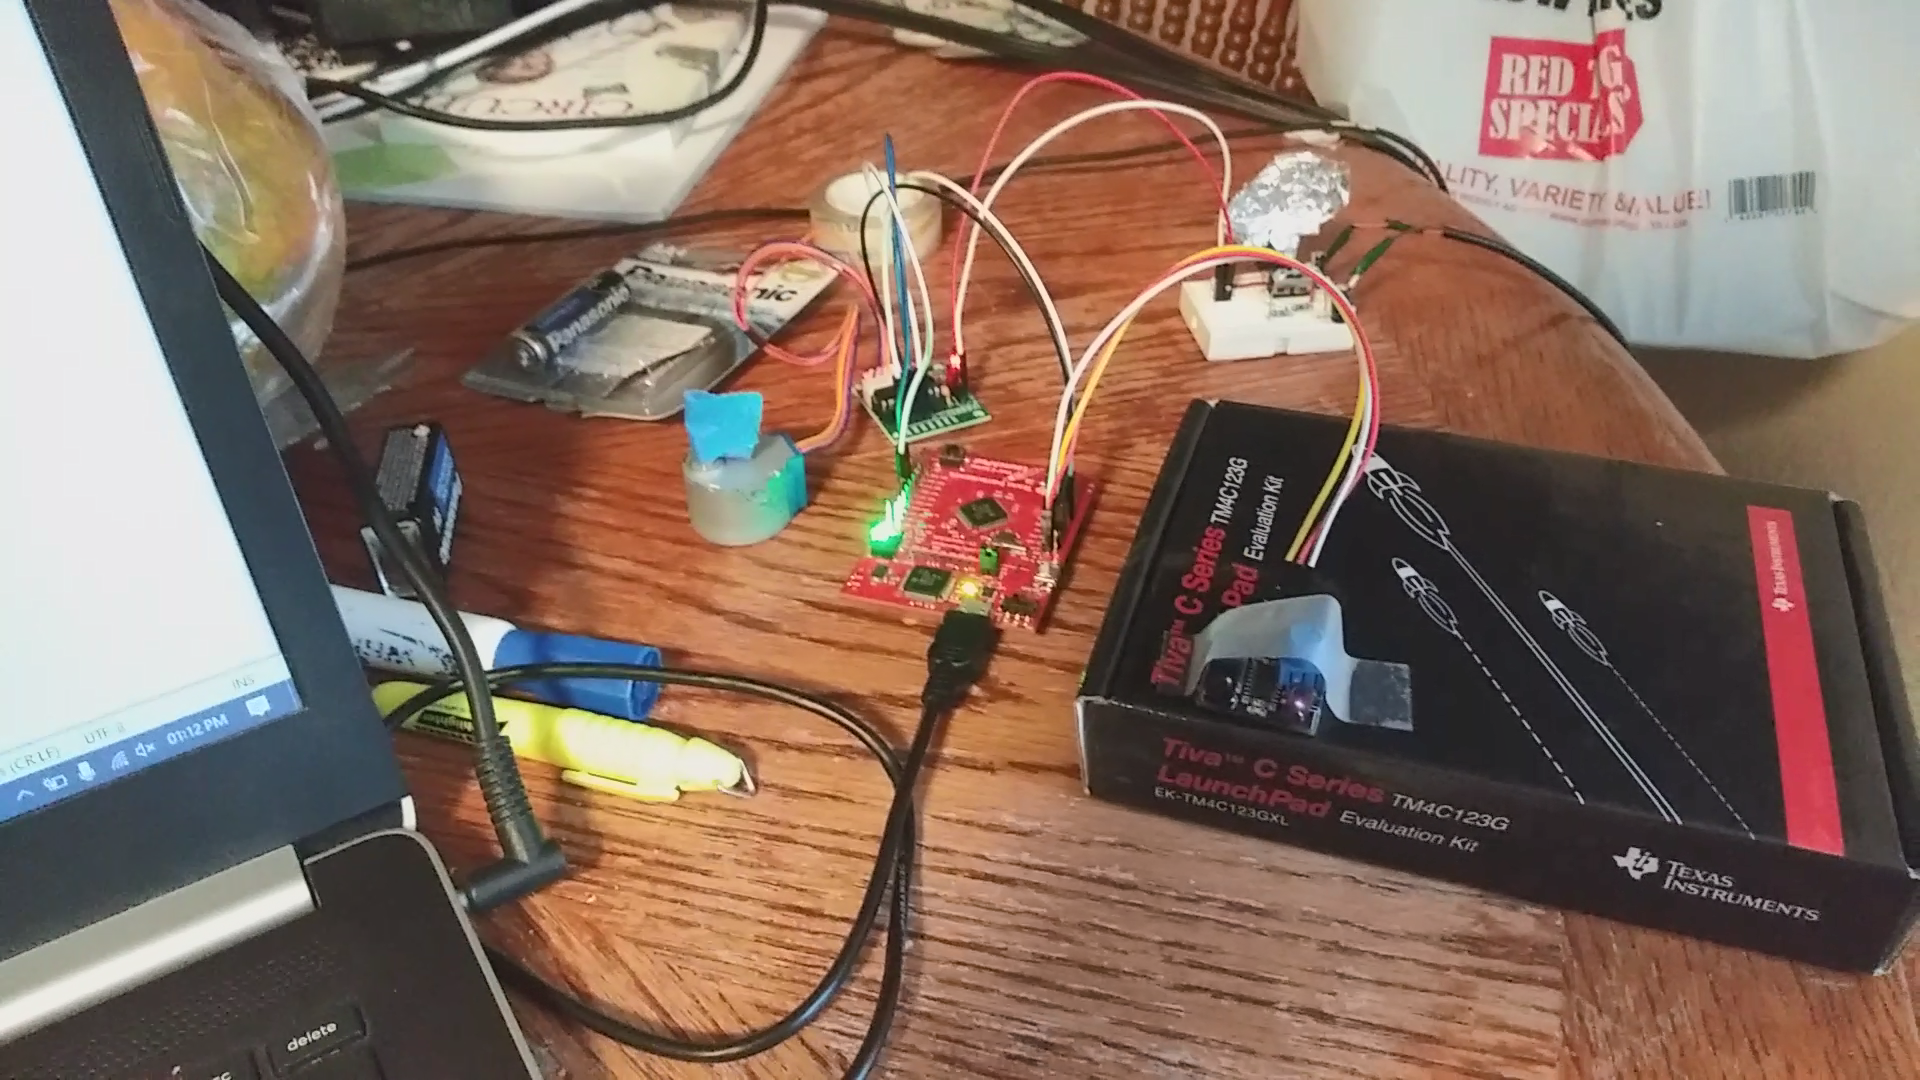
\includegraphics[width=\textwidth]{Images/image}
    \caption{Picture of system running.}
    \label{system}
\end{figure}

\section{Introduction} The goal of this project is to
extend the functionality of Lab 4 by adding a
stepper motor and changing some functionality, such as the
buttons. Specifically, the changes to Lab 4 are listed
below:

\begin{itemize}
    \item A stepper motor (28BYJ-48 driven by a ULN2003A
    Darlington transistor array) was added.
    \item \c{sw2} was removed and instead replaced with a
    toggle functionality for \c{sw1}.
    \item Timing for flashes adjusted slightly.
\end{itemize}

For more in-depth details about the rest of the functionality
of this project, please refer to the Lab 4 Report.

\section{Operation} As noted previously, the stepper
motor used for this project is the
28BYJ-48\footnote{\url{http://robocraft.ru/files/datasheet/28BYJ-48.pdf}}, a unipolar
stepper motor, which is driven by the ULN2003A(N)%
\footnote{\url{https://www.alldatasheet.com/datasheet-pdf/pdf/29528/TI/ULN2003AN.html}}
integrated circuit. The motor/driver system takes
in four signal inputs and a \SI{5}{V} power input. Its four
signal inputs are capable of driving the motor with only
\SI{8}{\milli\ampere} of current from the microcontroller's
GPIO ports.

For this project, if the state transitions from green to
blue, the motor will rotate a certain direction (say clockwise)
to symbolize a garage door opening or closing; if the state
transitions from blue to green, the motor will rotate the
opposite direction (say counterclockwise).

Making the stepper motor rotate is achieved using the
``wave-driving'' technique; this means that only one coil is
energized at a time, and the coil that is energized at any
given time is situated next to the coil that was previously
energized (coils 1 and 4 act as if they were next to each other).

The functionality for \c{sw2}
was removed; instead, a toggle functionality was added to \c{sw1}.
If the current state is green, pressing the button will
make the system transition to blue;
if the current state is blue, pressing the button will
make the system transition to green.

The link to a video demonstration of the system can be found
here: \url{https://youtu.be/S_4pRYOBeEA}.

\section{Theory} Instead of using a finite state machine
model for this project, I decided to go with a
straightforward procedural design. By doing it this way, I was
able to focus on the implementation of the stepper motor
instead of taking time to completely re-write Lab 4.
I was able to make a minimum number of changes in order to
get this project working. Figure \ref{fig:flowchart} shows
a flowchart of operation.

\begin{figure}[H]
    \centering
    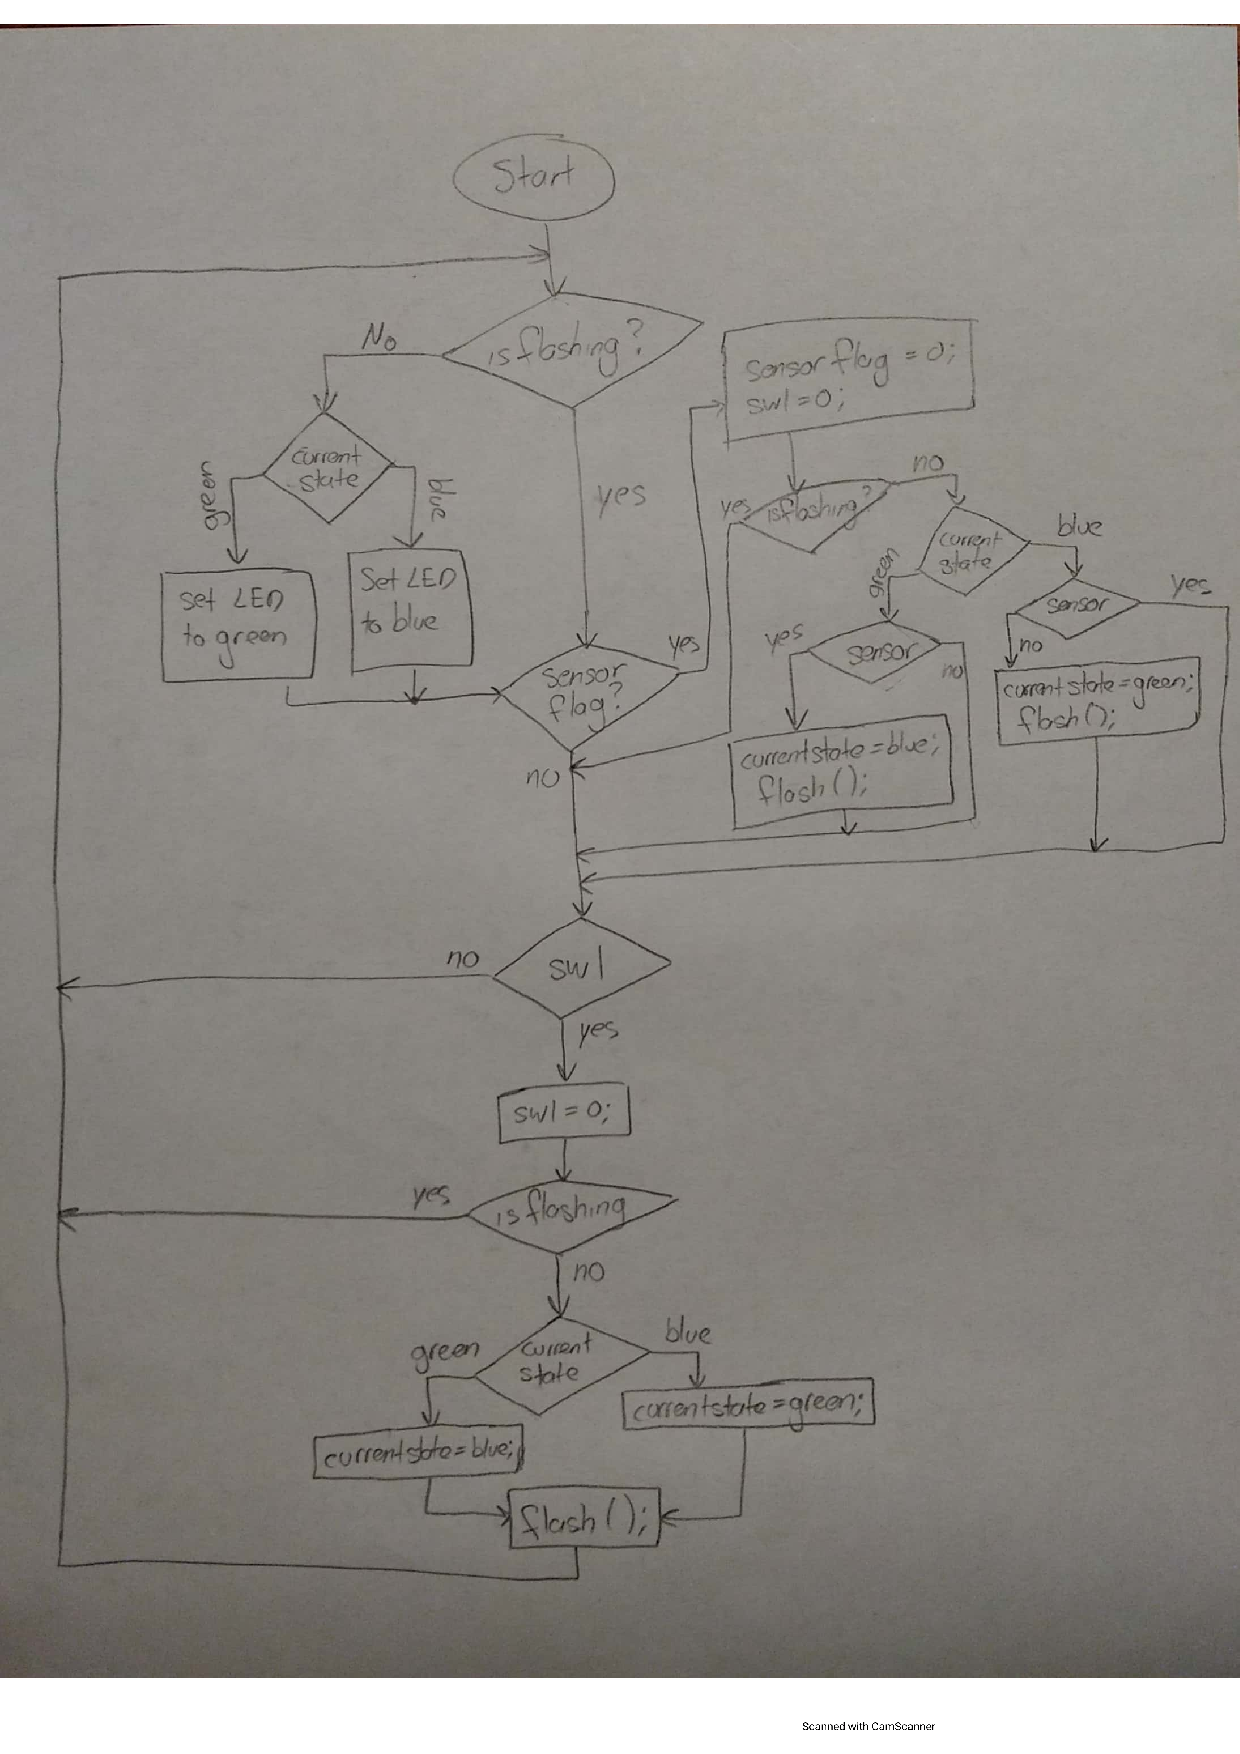
\includegraphics[width=\textwidth]{Images/flowchart}
    \caption{Flowchart of main operation.}
    \label{fig:flowchart}
\end{figure}

What is not shown in this flowchart are the \c{flash();}
function and how the flags get set. This is all implemented
using interrupts, so it does not happen in the main function,
and are implemented separately.

\section{Hardware Design} Just as before, the IR sensor is
connected to the same pins on the microcontroller. The difference
between Lab 4 and Project 2, however, is the addition of a
motor/driver combo. Four MCU outputs are dedicated to connecting
to the driver's inputs, and its outputs are connected to the
four stepper motor inputs. The motor/driver combo is externally
powered, to reduce the power of the microcontroller board.
It is necessary to output \SI{8}{\milli\ampere} of current
through the pins connected to the driver in order for the
driver to be effective.

\begin{figure}[H]
    \centering
    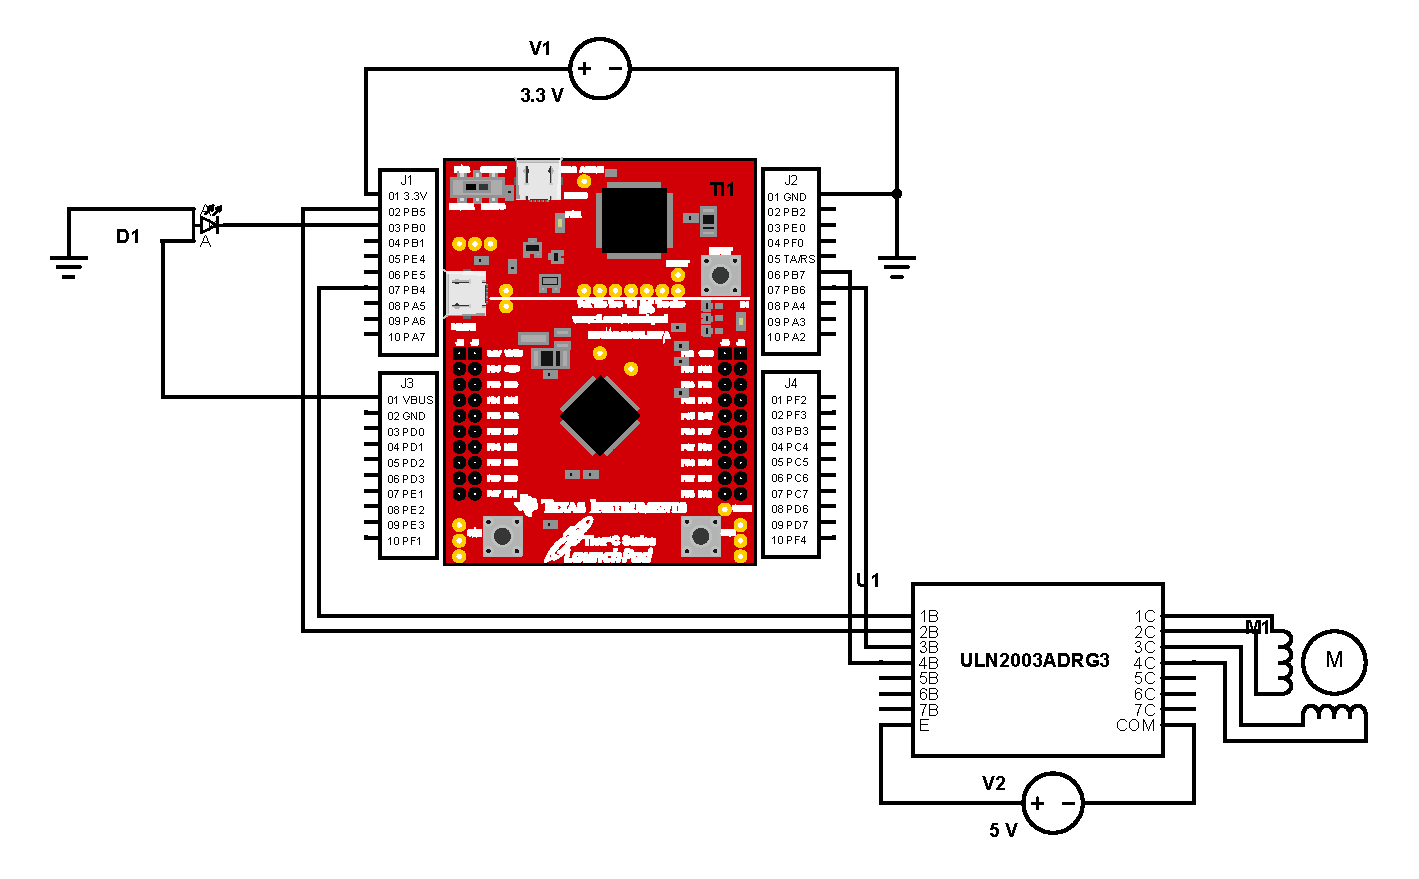
\includegraphics[width=\textwidth]{Images/schemeit-project}
    \caption{Schematic diagram of external connections.}
    \label{schematic}
\end{figure}

\section{Software Design} The flowchart for the software design
is presented in Figure \ref{fig:flowchart}. The basics are
copied over from Lab 4: using the SysTick timer, the
red light flashes at a frequency of \SI{4}{\hertz} while
the output for the motor changes every \SI{200}{Hz}. The
total amount of time spent flashing and rotating the motor
is \SI{5}{\second}. 

\section{Conclusion} This project, built from Lab 4, has helped
me learn about how a stepper motor is implemented, and how
you can get both precise angles and moderate speed using one.
I learned about the various ways one can drive the motor,
and their advantages and disadvantages.

\end{document}
